Synchronization of the GoPro cameras is essential for seamless orthophoto generation and boresight calculation.  The GoPro cameras do not have any documented methods to synchronize either video or imagery acquired with more than one camera.  A custom solution was developed to utilize the external microphone port of the GoPros in order to embed metadata in any recorded video files.  The approach using the audio port was selected, and is integrated in a modular manner, so that alternative video cameras with an external microphone option can be synchronized in the future using this same methodology.  
\section{Other Considered Methodology}
An alternative approach using a GoPro remote trigger was also investigated, but proved to be inadequate.  GoPro cameras can also be purchased with an external, handheld remote which operates over wifi to trigger one or more cameras.  This approach was investigated and tested for feasibility by triggering four GoPro cameras indoors.  The variable latency between when the remote was pressed and each GoPro began acquiring data was clearly discernable through the audible beep that each camera made when the command was received and acknowledged.  The audible beep variability between cameras was sometimes on the order of tenths of a second, which is far too great of an offset for accurate triggering.  Had the cameras been triggered at the exact same time, further investigation would have still been needed to ensure that there was no temporal drift between cameras. 

\section{Audio Encoding Technical Approach}
The methodology to time sync the imagery relies on the two audio channels (left and right) of the GoPro.  The left channel received the Binary counter integer once a second, and the right channel records the raw PPS from the GPS.  The Teensy microcontroller records the exact time it sent the binary signal to the GoPro.  This establishes a correspondence between the Teensy and GPS time frame.  The GPS also sends the PPS and GPS NMEA string to the Teensy, which can be used to solve for a time synchronized pointcloud to UTC time.

The binary signals sent to the GoPro are timestamped with the GoPro internal time, which is synchronized to the video frames that are being acquired.  These type of binary signals are normally decoded by a serial port, but a custom solution was developed to decode the information from the audio signal.  These signals are then decoded in pos- processing to synchronize the GoPro Video frames to GPS time.  This methodology only works when the GoPros are in video mode, and therefore the spatial resolution is limited compared to the image frame capture capabilities.

An initial approach to record raw NMEA sentences from a GPS receiver was unsuccessful due to difficulties in decoding the raw data, as well as bandwidth limitations.  A theoretical maximum of only 48kbs could be sent over each microphone channel due to the fixed sampling frequency of the GoPro microphone port, however in practice this value is much lower due to signal conditioning.  For this reason, an alternative approach utilizing a SD card for data logging was selected. 

A microcontroller is used as the system master, and it interfaces with a GPS receiver, a SD card logger, and the GoPro external microphone ports.  The microcontroller is constantly recording GPS NMEA data directly to the SD card, and logging it with an internal timestamp depicting when the GPS data was received.  Note that this timestamp certainly has some latency associated with it, as the timestamp is only recorded once the GPS has processed the raw signals and the microcontroller has acknowledged receipt of the serial data.  For this reason, the PPS signal is also recorded to both the SD card and the GoPro external right microphone channel.  This PPS, when coupled with the NMEA string, can provide accurate timestamping with nanosecond precision.  Due to the latency between video frames and audio recorded by the GoPro, as well as the interpolation between frames acquired at 30Hz, nanosecond precision can not be achieved with this methodology.  Further details on the processing of the GoPro audio and Teensy logfile to achieve timestamped video is explained in detail in Chapter \ref{ch:sync}.

\section{Component Selection}
The components for the PCB were selected to minimize space, weight, and power requirements.  The following components were selected and integrated onto the PCB, and a short description of the part is provided.
\subsection{Teensy 3.2}

\url{https://www.pjrc.com/teensy/teensy31.html}\vspace{0.5em}

The Teensy 3.2 microcontroller is a 32bit, breadboard friendly microcontroller that operates on 3.3V logic.  It was selected mainly due to the small form factor and access to the three Serial ports required for interfacing with the SD card, GPS, and GoPro camera.  Compared to Arduino brand microcontrollers with similar capabilities, the Teensy 3.2 is also lower cost and has increased performance.  The Teensy can be programmed with the Arduino IDE, so the transition from Arduino code used in previous iterations of the sensor to the Teensy was seamless.  
\subsection{openLog}

\url{https://www.sparkfun.com/products/9530}\vspace{0.5em}

The openLOG is a lightweight, easy to implement data logger that takes any serial data passed to the RX port and logs it to a microSD card.  The SD card is initially set to a default 9600 baud rate, but the config.txt file on the sd card is modified for this project so that it logs at 115200.  The SD card must have the config.txt file with the baud rate field set to 115200 for the current code to work.
\subsection{Adafruit Ultimate GPS}

\url{https://www.adafruit.com/products/746}\vspace{0.5em}

The Ultimate GPS is a low cost L1 only GPS receiver that has a PPS output.  It was selected because it is low cost, lightweight and easy to integrate as it has the digital io pins broken out to headers.  The PPS pin in conjunction with the NMEA GPS string provides accurate timestamping of the imagery, as well as a low quality GPS position.
\subsection{Voltage Regulator}

\url{https://www.adafruit.com/products/1065}\vspace{0.5em}

The ``Mini DC-DC 5V Stepdown'' regulator was chosen as it provides up to 94\% efficiency and up to 1A output.  It also has a 6.5-32V input range, which allows for various battery options to be explored.  The high efficiency of the DC-DC stepdown enables smaller and lighter batteries to be used.
\subsection{9 Degree of Freedom IMU}

\url{https://www.sparkfun.com/products/13284}\vspace{0.5em}

The LSM9DS1 is a 9 degree of freedom motion sensing chip that houses a triad of accelerometers, gyroscopes, and magnetometers.  This Chip was selected as it is very lightweight, low cost, and should contain the ability to generate low accuracy camera poses.  It communicates via I2C protocol, and therefore an extra serial port is not required.
\subsection{JST Connectors}

\url{https://www.sparkfun.com/products/9916}\vspace{0.5em}

JST connectors are a brand of connector that connects a breadboard to a cable.  These are purchased with the wires already broken out for ease of integration in 2-pin, 3-pin, and 4-pin connector packages.  
\subsection{``SuperBright" LEDs}

\url{https://www.adafruit.com/products/754}\vspace{0.5em}

LED status lights were selected to be as bright as possible because previous data status LEDs were difficult to view in bright, outdoor lighting.  These status lights use more battery, but as they are dubbed "superbright", they are much easier to see.  The polarity of the pins of the LED are important, and are depicted by the length of the wire to the LED.  The longer wire is the positive lead, and the shorter is the negative, as depicted in \figref{fig:led}.  

\begin{figure}[h]
	\centering
	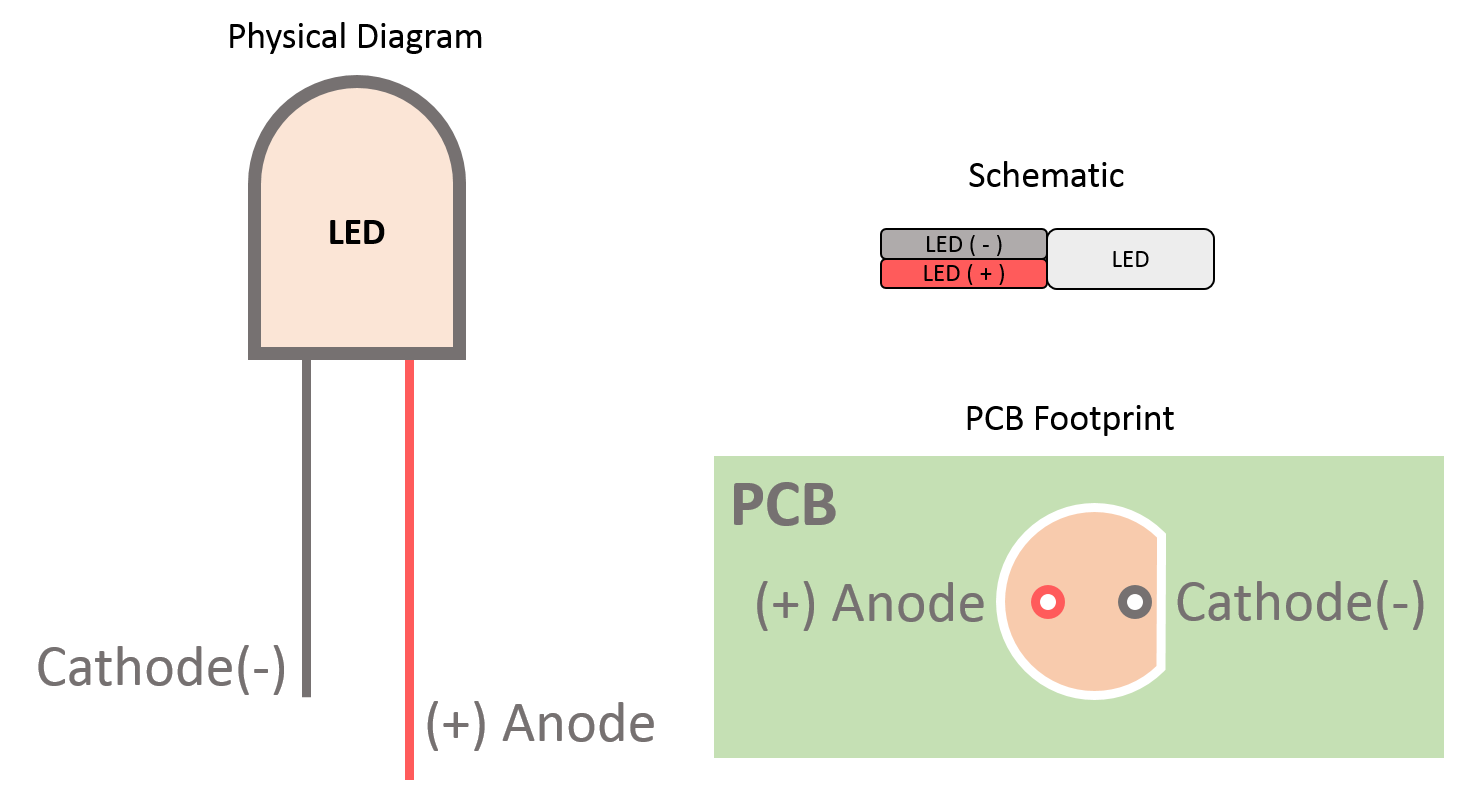
\includegraphics[width = .75\linewidth]{../figures/LED.png}
	\caption{The LEDs used are follow a traditional LED diagram and PCB format, where the longer wire represents the Anode.}
	\label{fig:led}
\end{figure}

\section{PCB Schematics and Board Designs}
EAGLE was used to generate the schematic and board designs for the circuit.  The design was divided into two PCBs.  The first PCB, referred to as the ``Main'' PCB, contains all of the main components of the circuit.  The second PCB, referred to as the ``Panel'' PCB, works as a connector so that the GoPro cables can be connected and disconnected easily from the outside.  
\subsection{Main PCB}
The schematic for the main PCB, shown in \figref{fig:schematic}, is divided into the Power, Voltage Divider, Optional LEDs, Camera Output, Teensy microcontroller and Sensors sections.  Notice that in the Voltage Divider section, in order to ensure the correct Voltage levels into the GoPro microphone port a voltage divider was used to reduce the 3.3V input to approximately 30mV for both the PPS and NMEA ports. 

\begin{figure}[h]
	\centering
	\includegraphics[width = .75\linewidth]{../figures/Schematic.png}
	\caption{The main schematic was designed in EAGLE, and a higher resolution is available in the deliverables folder structure as both a ".sch" and ".png" file.}
	\label{fig:schematic}
\end{figure}

The main board layout, shown in \figref{fig:board}, was designed to minimize the footprint and reduce large cable bending by placing connectors near the edge of the board.  The board was also designed in conjunction with the 3D printed mount, and the shape and orientation was optimized to fit on the electronics tray.  The order that the components are soldered is important such that nothing covers up something that needs to be soldered from the other side of the board.

\begin{figure}[H]
	\centering
	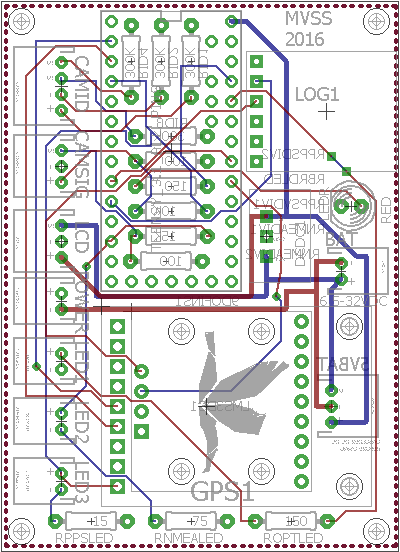
\includegraphics[height = 2in]{../figures/board.png}
	\caption{The main board layout was designed in EAGLE. Red traces represent the top of the board and blue traces represent the bottom.}
	\label{fig:board}
\end{figure}
\subsection{Panel PCB}
The Panel PCB serves as a connection point for the cables that go to the GoPro.  The main PCB outputs the ground signal, two ``pseudo-audio'' signals, and an ``ID'' wire for each camera.  The ground, as well as the PPS and binary ``pseudo-audio'' signals are split into 4 signals each so that the signal can be sent to each of the four cameras.  The ID signals are individually sent to each camera, as the 300k$\Omega$ resistor tying the signal to ground is what tells the goPro to store audio from the ``external audio'' port.  The schematic is shown in \figref{fig:panelschematic}, and the board is shown in \figref{fig:panelboard}.
\begin{figure}[H]
	\centering
	\includegraphics[height = 2in]{../figures/panelZoomschematic.png}
	\caption{The panel schematic was designed in Eagle. This simple PCB is used as a connector so that the 7 signals are split to go to the 16 signals required for the GoPro.}
	\label{fig:panelschematic}
\end{figure}
\begin{figure}[h]
	\centering
	\includegraphics[height = 1in]{../figures/panelboard.png}
	\caption{The panel board layout was designed in EAGLE. Red traces represent the top of the board and blue traces represent the bottom.}
	\label{fig:panelboard}
\end{figure}

\section{Cable Pin Labels}
The pinouts for each of the two PCBs are depicted in \figref{fig:pinouts}.  These cables should be custom made to the correct length so as to reduce the overall weight of the system.  Each of the JST connectors comes with the leads already crimped into the connector and tinned with solder on the other end.  This allows for them to be easily soldered together to generate a solid connection.  
\begin{figure}[H]
	\centering
	\includegraphics[scale = 0.5]{../figures/pinoutmainPCB.pdf}
	\includegraphics[scale = 0.5]{../figures/pinoutpanelPCB.pdf}
	\caption{The pinouts for the main PCB and panel PCB are labeled.  The color of the box represents the color of the wire. }
	\label{fig:pinouts}
\end{figure}

\section{GoPro Mini-USB-B Cable}
The cable that connects the GoPro to the PCB is based on a USB mini-B cable with 10 pins.  It utilizes the pins as shown in \tabref{tab:pinouts}.  The 300k$\Omega$ resistor could have been placed within the cable, or immediately after the socket, as both channel 7 and 3 are right next to each other and a resistor could simple be soldered across the two.  This would reduce the number of wires in the cable from 4 to 3.  However for this version of the cable the resistor is placed on the PCB rather than in the cable to improve the ability to debug the system.  

\begin{table}[h]
	\centering
	\begin{tabular}{l|l}
		\toprule
		Pin Number & Description \\
		\midrule
		Pin 3 & Ground\\
		Pin 4 & Right Audio Channel\\
		Pin 5 & Left Audio Channel\\
		Pin 7 & ID pin which enables the external audio when brought to ground across a 300k$\Omega$ resistor.\\
		\bottomrule
	\end{tabular}
	\caption{The GoPro cable utlizes pins 3,4,5, and 7 to trigger the camera via the audio port.}
	\label{tab:pinouts}
\end{table}

\begin{figure}[H]
	\centering
	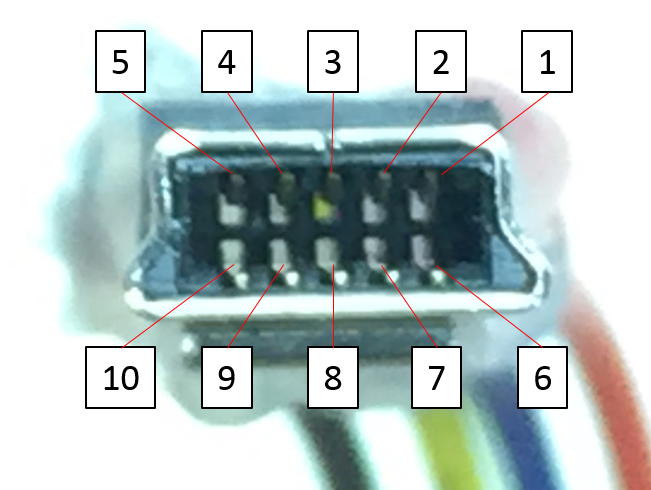
\includegraphics[scale = 0.7]{../figures/tenpin.png}
	\caption{Traditional cables that are purchased in retail stores only break out 4 of the 10 pins in a mini-B connector.  The GoPro triggering cable requires a custom cable, as pins 3,4,5 and 7 are used.}
	\label{fig:pinouts}
\end{figure}

\section{Power}
The power input into the PCB is set up for 6.5V - 32V DC by default, with a maximum output of 1A at 5V.  The average current draw was tested for a 9V battery. The average power draw is calculated using \eqnref{eqn:PVI} shown in \tabref{tab:avgPower}, and estimated runtime calculated with with \eqnref{eqn:estbat} different batteries is shown in \tabref{tab:batRuntime}.
\begin{equation}
\label{eqn:PVI}
Average\hspace{.5em} Power = Voltage \times Current
\end{equation}
\begin{table}[H]
	\centering
	\begin{tabular}{lcr}
		\toprule
		Average Voltage (V) & Average Current (mA) & Average Power (W) \\
		\midrule
		8.3 & 0.080 & 0.664 \\
		\bottomrule
	\end{tabular}
	\caption{The average power draw for the PCB was calculated using a 9V battery.}
	\label{tab:avgPower}
\end{table}

\begin{equation}
\label{eqn:estbat}
Estimated\hspace{.5em}Runtime (hours) = \frac{Battery\hspace{.5em} Voltage \times Battery\hspace{.5em} Current}{Average\hspace{.5em} Power} 
\end{equation}
\begin{table}[H]
	\centering
	\begin{tabular}{lccr}
		\toprule
		Battery Type & Voltage & Estimated Capacity(mah) & Estimated runtime(hours) \\
		\midrule
		9V Battery & 9 & 400 & 5.4\\
		Two 1000mA Lithium Ion & 7.4 & 1000  & 11.1\\
		Three 1000mA Lithium Ion & 11.1 & 1000  & 16.7\\
		\bottomrule
	\end{tabular}
	\caption{The estimated runtime is calculated for a number of potential battery options.}
	\label{tab:batRuntime}
\end{table}
\subsection{Alternate Power}
An alternate method for powering the PCB is provided via a 3-Pin JST connector on the bottom of the board.  The pinout for this port is not documented, as it has not been tested.  The board and schematic should be read to determine the proper power input values.  The connector provides the user access to provide their own regulated 5V battery circuit.  There is one wire for ground, one for 5V, and another for raw voltage.  The raw voltage line is used to monitor battery status and health using the LCD on the front of the panel.

\section{Microcontroller Algorithm}\label{sec:algoLog}
The algorithm to write the logfile to the SD card is programmed using the Arduino IDE.  The Arduino IDE is used as the programming environment for the Teensy, per documentation on the Teensy website.  A flowchart depicting the code is shown in \figref{fig:TeensyFlow}, and the code is provided in electronic form.  Emphasis is placed on ensuring accurate timing, but precedence is placed in this order:
\begin{enumerate}
	\item Accurate retrieval of Teensy time when PPS rising edge is detected
	\item Accurate Teensy time of when counter was sent to gopro
	\item Accurate Teensy time of when the GPS time is received
\end{enumerate}
The three different time references that are used for time syncing are GoPro time, Teensy time, and GPS time.  GoPro time is the internal time of the GoPro camera in seconds from the time the video began recording.  Teensy time is the time in milliseconds since the Teensy was powered on.  GPS time is the Coordinated Universal Time(UTC), which is output from the GPS.  The synchronization between these times is described in more detail in Chapter \ref{ch:sync}, but it is essential that the times are recorded as precisely as possible.  

To ensure that the PPS and Teensy time are accurately correlated, an interrupt routine is implemented in the Teensy algorithm.  An interrupt routine, while technically different than running in parallel, can essentially be seen as a parallel processing task.  In this algorithm, the interrupt is constantly monitoring for the rising edge of the PPS pulse.  When the rising PPS pulse is detected, the code stops whatever it is doing and jumps directly into the interrupt routine.  The interrupt records the exact Teensy time when this occured, and saves it to a global variable before releasing the code to finish performing whatever task it was working on.  It then writes the data to the SD card whenever it is convenient, as once the exact Teensy time is recorded there is no urgency to write the data.  

\begin{figure}[H]
	\centering
	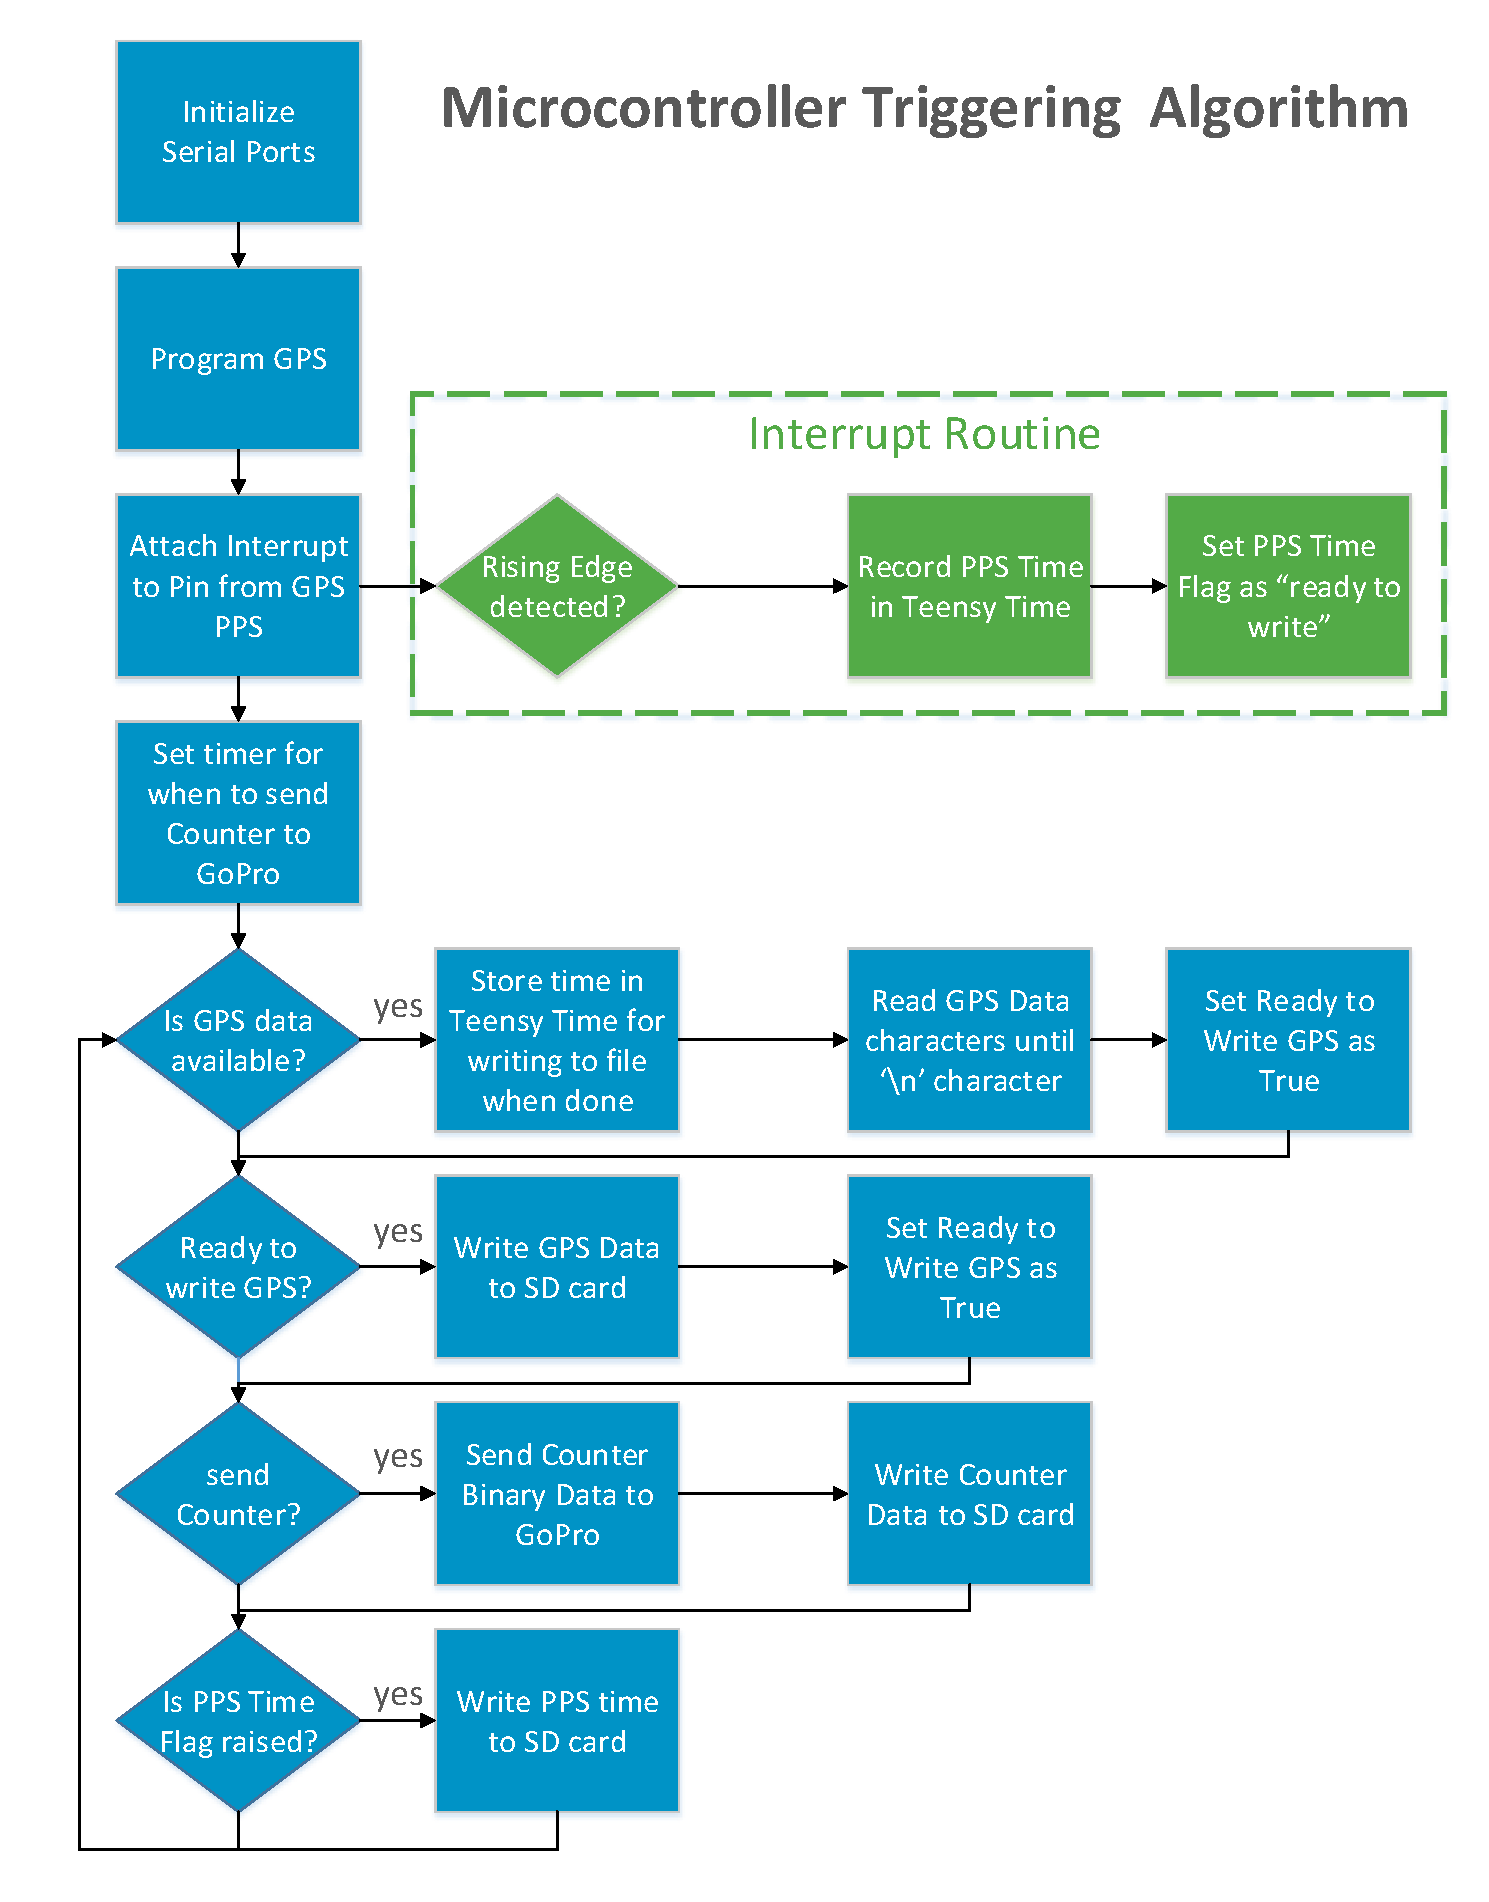
\includegraphics[scale = 0.4]{../figures/TeensyFlowchart.pdf}
	\caption{The Teensy algorithm is written to attempt to ensure as accurate timing synchronization as possible.  }
	\label{fig:TeensyFlow}
\end{figure}

The output log file is structured similarly to the NMEA format, but does not enact checksums for each line.  Each line of data is sent as a comma delimited line, where the first column is the address field, or identifier preceded by a `\$'.  The second column in each line is always the time in milliseconds from the time the microcontroller was turned on.  The relevant id fields are described in \tabref{tab:nmea}.  An example snippet of data from the file is shown in \figref{fig:nmea}.  A script for parsing the data is shown in \algref{alg:getValue}.
 \begin{table}[h]
 	\centering
 	\begin{tabular}{ll}
 		\toprule
 		ID & Description \\
 		\midrule
		\$MSG & Any Raw GPS NMEA Strings \\
		\$IND & Counter number that was sent to the GoPro \\
		\$PPS & No Info, besides the time it was received at \\
 		\bottomrule
 	\end{tabular}
 	\caption{The ID for each log file line is essential to parsing the data.}
 	\label{tab:nmea}
 \end{table}
 
 \begin{figure}[H]
 	\centering
 	\includegraphics[scale = 0.7]{../figures/logfileend.png}
 	\caption{The Teensy log file is recorded similarly to a NMEA structure, with each line beginning with an ID preceded by a `\$' symbol, and followed by the time in Teensy time.}
 	\label{fig:nmea}
 \end{figure}

\section{Potential Electronics Improvements}
\subsection{Fix Blunders in PCB Board}
There are a few improvements that could be made to the PCB and electronics for future versions.  The first improvement is an improved main PCB.  The PCB design used for this version had a few minor errors.  These error included: the DC-DC having to be mounted backwards, a slight offset of the IMU pins, and a few incorrect resistor values.  These fixes were manually implemented when the PCB was soldered together, and also electronically implemented in the board and schematic diagrams.  The new files are saved and have been delivered electronically.  
\subsection{Integrate onboard IMU}
The IMU is soldered to the board and connected to the SDA and SCL ports, however it is currently unrecorded.  The initial focus was to ensure accurate timestamping before adding in more read write cycles from the IMU.  While this IMU is very low cost, and low accuracy, it will most likely be able to provide a rough estimate of camera orientation.  
\subsection{Improve GPS Quality}
A large improvement would be to improve the quality of the GPS receiver.  The current L1 only GPS is accurate to less than 3m per the documentation, and does not record raw pseudo-ranges for post-processing.  Integration of a RTK GPS, L1 and L2 GPS, post-processing enabled GPS, or a fully integrated INS would greatly benefit the calculation of the camera pose and orientation.  The Ultimate GPS is placed into a socket on the PCB, with the thought that in the future an improved GPS sending NMEA strings could be integrated into the workflow with possibly only software modifications.
\subsection{Implement Charge Port and USB Hub}
A final improvement could be implemented to improve the usability of the system by adding a charge port and a USB hub to enable charging and reading from the sensors via one cable.  The current workflow for getting data out of the system involves removing the SD card or plugging a separate USB cable into the USB port.  An integrated switch on the Panel PCB could be a good place for a USB hub or a battery charging circuit.